\section{Evaluation}\label{sec:eval}

To evalute feature-sensitive coverage criteria, we apply $\tool$ to the latest
language specification (ES13, 2022)~\cite{es13} to synthesize JavaScript
conformance tests.
%
Our tool synthesizes 237,981 conformance tests in 50 hours using $\tool$ with
five different graph coverage criteria: 1) 0-FS, 2) 1-FS, 3) 2-FS, 4) 1-FCPS,
and 5) 2-FCPS node-or-branch coverage.
%
We performe our experiments with five Ubuntu machines with a 4.0GHz Intel(R)
Core(TM) i7-6700k and 32GB of RAM (Samsung DDR4 2133MHz 8GB*4).

%----------------------------------------%

Using the synthesized JavaScript conformance tests, we check the conformance of
eight mainstream implementations (four engines and four transpilers) listed in
Table~\ref{tab:conform-bugs}.
%
We select them as evaluation targets because they support all the language
features in ES13;
%
V8, JSC, and SpiderMonkey are JavaScript engines used in web browsers, Google
Chrome, Apple Safari, and Mozilla Firefox, respectively.
%
GraalJS is a JavaScript engine built on GraalVM, a JDK distribution developed by
Oracle written for JVM languages along with support for cloud-native and
polyglot.
%
Babel and SWC are transpilers that desugar new language features into old ones,
usually ES5.1 features, for legacy host environments.
%
Terser is a code compressor that reduces the code size by removing code
fragments, making names smaller, or inlining variable references.
%
Finally, JavaScript Obfuscator obfuscates code to make it hard to understand and
reverse-engineering.
%
For the transpiler conformance check, we use the V8 engine as the default engine
to execute the transpiled code with assertions.
%
If a test fails in V8, we search for another engine that passes the test and use
it for the transpiler conformance check.
%
However, we do not use the test for transpiler conformance check if it fails on
all engines.

%----------------------------------------%

We evaluate the synthesized conformance tests using our feature-sensitive
coverage criteria with the following four research questions:
\begin{itemize}
  \item \textbf{RQ1 (Conformance Bug Detection):} How many conformance bugs are
    detected in JavaScript implementations by synthesized conformance tests?
    (Section~\ref{sec:conform-bug})
  \item \textbf{RQ2 (Impact of $k$-FS Coverage Criteria):} Are $k$-FS coverage
    criteria effective in detecting conformance bugs?
    (Section~\ref{sec:impact-k-fs})
  \item \textbf{RQ3 (Impact of $k$-FCPS Coverage Criteria):} Are $k$-FCPS
    coverage criteria more effective than $k$-FS coverage criteria in detecting
    conformance bugs? (Section~\ref{sec:impact-k-fcps})
  \item \textbf{RQ4 (Comparison with Test262):} Can conformance tests
    synthesized by $\tool$ improve Test262, the official JavaScript conformance
    suite maintained by hand? (Section~\ref{sec:compare-test262})
\end{itemize}

%----------------------------------------%
%----------------------------------------%

\subsection{Conformance Bug Detection}\label{sec:conform-bug}

\begin{table}
\caption{
  Detected conformance bugs in JavaScript engines and transpilers.
}
\vspace*{-.5em}
{
\footnotesize
\label{tab:conform-bugs}
\begin{tabular}{?c?l|l|l?r|r|r?}
\toprule\\[-1.6em]

\multicolumn{1}{?c?}{\multirow{2}{*}{\textbf{Kind}}}
& \multicolumn{1}{c|}{\multirow{2}{*}{\textbf{Name}}}
& \multicolumn{1}{c|}{\multirow{2}{*}{\textbf{Version}}}
& \multicolumn{1}{c?}{\multirow{2}{*}{\textbf{Release}}}
& \multicolumn{3}{c?}{\textbf{\# Detected Unique Bugs}} \\\cline{5-7}

&&&
& \multicolumn{1}{c|}{\textbf{\# New}}
& \multicolumn{1}{c|}{\textbf{\# Confirmed}}
& \multicolumn{1}{c?}{\textbf{\# Reported}}\\

\toprule\\[-1.6em]

\multirow{5}{*}{Engine}
& V8            & v10.8.121 & 2022.10.06 & \x{0} & \x{0} & \x{2} \\\cline{2-7}
& JSC           & v615.1.10 & 2022.10.26 & \x{8} & \x{8} & \x{12}\\\cline{2-7}
& GraalJS       & v22.2.0   & 2022.07.26 & \x{9} & \x{9} & \x{9} \\\cline{2-7}
& SpiderMonkey  & v107.0b4  & 2022.10.24 & \x{1} & \x{2} & \x{3} \\\cline{2-7}
& \multicolumn{3}{c?}{\textbf{Total}}    & \y{18}& \y{19}& \y{24}\\

\toprule\\[-1.6em]

\multirow{5}{*}{Transpiler}
& Babel         & v7.19.1   & 2022.09.15 & \x{27}& \x{27}& \x{31}\\\cline{2-7}
& SWC           & v1.3.10   & 2022.10.21 & \x{22}& \x{22}& \x{37}\\\cline{2-7}
& Terser        & v5.15.1   & 2022.10.05 & \x{1} & \x{1} & \x{15}\\\cline{2-7}
& Obfuscator    & v4.0.0    & 2022.02.15 & \x{0} & \x{0} & \x{5} \\\cline{2-7}
& \multicolumn{3}{c?}{\textbf{Total}}    & \y{50}& \y{50}& \y{83}\\

\toprule\multicolumn{1}{c}{}\\[-1.6em]


\multicolumn{4}{?c?}{\textbf{Total}}
& \y{69}& \y{69}& \y{107}\\

\toprule\multicolumn{1}{c}{}\\[-1.6em]
\end{tabular}
}
\end{table}

%----------------------------------------%

Table~\ref{tab:conform-bugs} gives the distribution of the detected conformance
bugs by 237,981 synthesized conformance tests.
%
We found conformance bugs in all the evaluation targets using the synthesized
conformance tests.
%
In addition, we manually inspected the failed conformance test cases,
categorized them as \inred{107} distinct conformance bugs, and reported them to
the developers of implementations.
%
As a result, \inred{69} out of \inred{107} bugs were officially confirmed, and
\inred{68} were newly discovered bugs.
%
The other \inred{38} reported bugs are still under review, or developers have
not yet responded.
%
Among \inred{107} detected bugs, \inred{24} are engine bugs, and \inred{83} are
transpiler bugs.
%
Now, we intorudce interesting bugs detected by our synthesized conformance
tests in eight implementations.

%----------------------------------------%

\paragraph{\textbf{Order of Execution}}
%
JavaScript engines must follow the execution order of each language feature
described in the language specification.
%
However, we detected a severe bug\footnote{
  We anonymized links of bug reports for double-blinded reviewing.
  % TODO during camera-ready
  % https://github.com/oracle/graaljs/issues/655
  % https://github.com/oracle/graaljs/issues/671
} related to the execution order of \jscode{delete} operation that causes
the exeuction of originally unreachable code in the GraalJS engine.
%
For example, while the following code should return \jscode{false}, it throws an
exception with \jscode{"ERR"} by executing the originally unreachable code
inside the arrow function in GraalJS:
%
\begin{lstlisting}[style=JS, basicstyle=\footnotesize\ttfamily]
false && delete (() => { throw "ERR"; })(); // Expected: false
\end{lstlisting}
%
In addition, we detected another bug\footnote{
  We anonymized links of bug reports for double-blinded reviewing.
  % TODO during camera-ready
  % V8 - https://bugs.chromium.org/p/v8/issues/detail?id=13469
  % GraalJS - https://github.com/oracle/graaljs/issues/673
  % JSC - https://bugs.webkit.org/show_bug.cgi?id=247723
  % SpiderMonkey - https://bugzilla.mozilla.org/show_bug.cgi?id=1800062
  % ECAM-262 - https://github.com/tc39/ecma262/issues/2659
} related to the execution order of property read in the V8 engine.
%
% For example, while the following code should throw an exception with
% \jscode{"ERR"}, V8 throws a \textbf{TypeError} exception:
%
% \begin{lstlisting}[style=JS, basicstyle=\footnotesize\ttfamily]
% null [ { [Symbol.toPrimitive ] : () => { throw "ERR"; } } ];
% \end{lstlisting}
%
More interesting point is that all target engines contain this conformance bugs.
%
Thus, ECMA-262 may have to be updated based on majority of the semantics used in
the implementations.

%----------------------------------------%

\paragraph{\textbf{Asynchronous Function / Generator}}
One of the complex language features in JavaScript is asynchronous functions and
generators introduced in ES6 (2015).
%
We detected a severe bug\footnote{
  We anonymized links of bug reports for double-blinded reviewing.
  % TODO during camera-ready
  % https://github.com/tc39/proposal-async-await/issues/60
  % https://bugzilla.mozilla.org/show_bug.cgi?id=1799288
} in the SpiderMonkey engine that breaks the logic of asynchronous function
calls.
%
For example, the following code must return a rejected \jscode{Promise} object
because a non-iterable value \jscode{undefined} is assigned to an array
destructuring pattern \jscode{[]} in \jscode{async} arrow function:
%
\begin{lstlisting}[style=JS, basicstyle=\footnotesize\ttfamily]
(async function ([]) {})(); // Expected: A rejected Promise object
\end{lstlisting}
%
However, it unexpectedly terminates with a \textbf{TypeError} exception in 
the SpiderMonkey engine.
%
According to a developer of SpiderMonkey, it happens because no test is added to
Test262 after changing the semantics of \jscode{async} functions.
%
{
  \small
  \begin{quote}
    The async-function spec was changed at some point \textelp{}
    this is also not covered by test262.
  \end{quote}
}
%
% We also detected other similar bugs related to generators in the SWC transpiler,
% and its main developer appreciated our work and requested us to apply our tool
% for SWC using the \scode{jsc.minify} option as well.\footnote{
%   We anonymized links of bug reports for double-blinded reviewing.
%   % TODO during camera-ready
%   % https://github.com/swc-project/swc/issues/6375
% }

%----------------------------------------%
% \paragraph{\textbf{JSC}}
% %
% For JSC, we detected a conformance bug related to the order of properties for
% \jscode{class} expressions.
% % https://bugs.webkit.org/show_bug.cgi?id=247429
% In the following code, the variable \jscode{order} should be an array
% \jscode{["length", "name", "prototype"]}:
% \begin{lstlisting}[style=JS, basicstyle=\footnotesize\ttfamily]
% class C { static D = class {}; } let order = Reflect.ownKeys(C.D);
% \end{lstlisting}
% %
% However, it becomes \jscode{["length", "prototype", "name"]} in JSC.
% %
% This conformance bug is a hard-to-find bug because it is reproducible only when
% a \jscode{class} expression is assigned to a static field of another
% \jscode{class} declaration or expression.

%----------------------------------------%

% %
% Based on our bug reports, the developers of the Babel transpiler realilzed that
% Babel have many \textit{temporal dead zone (TDZ)} bugs caused by \jscode{let} or
% \jscode{const}.
% % https://github.com/babel/babel/issues/15150
% % (EXAMPLE) let x = x;
% % (EXAMPLE with TDZ option) const x = 0; x = 1;
% Thus, they created a special label \name{Spec: TDZ} to highlight issues related
% to TDZ bugs and started to fix bugs related to TDZ bugs.

%----------------------------------------%
%----------------------------------------%

\subsection{Impact of $k$-FS Coverage Criteria}\label{sec:impact-k-fs}

\begin{table}
\caption{
  Comparison of synthesized conformance test suite guided by five different
  graph coverage criteria: 1) 0-FS, 2) 1-FS, 3) 2-FS, 4) 1-FCPS, and 5) 2-FCPS
  node-or-branch coverage criteria.
}
\vspace*{-.5em}
{
\footnotesize
\label{tab:compare}
\begin{tabular}{?c?r|r|r?r|r?}
\toprule\\[-1.6em]

\multicolumn{1}{?c?}{\multirow{2}{*}{\textbf{Coverage Criteria} $\cov{\graph}$}}
& \multicolumn{3}{c?}{\textbf{\# Covered $k$-F(CP)S-TR (k)}}
& \multicolumn{1}{c|}{\multirow{2}{*}{\textbf{\# Syn. Test}}}
& \multicolumn{1}{c?}{\multirow{2}{*}{\textbf{\# Bug}}}\\\cline{2-4}

& \multicolumn{1}{c|}{\textbf{\# Node}}
& \multicolumn{1}{c|}{\textbf{\# Branch}}
& \multicolumn{1}{c?}{\textbf{\# Total}}
&&\\

\toprule\\[-1.6em]

0-FS node-or-branch (\sname{0-fs})
& 10.0    & 5.6     & 15.6    & 2,111  & 56  \\\hline
1-FS node-or-branch (\sname{1-fs})
& 79.3    & 45.7    & 125.0   & 6,766  & 84  \\\hline
2-FS node-or-branch (\sname{2-fs})
& 1,199.8 & 696.3   & 1,896.1 & 97,423 & \x{76} \\\hline
1-FCPS node-or-branch (\sname{1-fcps})
& 179.7   & 97.6    & 277.3   & 9,092  & 88  \\\hline
2-FCPS node-or-branch (\sname{2-fcps})
& 2,323.1 & 1,297.6 & 3,620.7 & 122,589& \x{67} \\

\toprule\multicolumn{1}{c}{}\\[-1.6em]

\end{tabular}
}
\end{table}

%----------------------------------------%

Table~\ref{tab:compare} shows the result of conformance test synthesis via
$\tool$ with five different graph coverage criteria: 1) 0-FS, 2) 1-FS, 3) 2-FS,
4) 1-FCPS, and 5) 2-FCPS node-or-branch coverage criteria.
%
Note that 0-FS node-or-branch coverage criterion is same with the node-or-branch
coverage criterion.
%
To evaluate the impact of $k$-FS coverage criteria, we compare the synthesized
conformance tests guided by different $k$-FS normal-or-branch coverage criteria
(\sname{0-fs}, \sname{1-fs}, and \sname{2-fs} in Table~\ref{tab:compare}).
%
The first three columns denote the number of covered $k$-FS- or $k$-FCPS-TRs for
nodes (\textbf{\small \# Node}), branches (\textbf{\small \# Branch}), and both
(\textbf{\small \# Total}).
%
The fourth and fifth columns denote the number of synthesized conformance tests
(\textbf{\small\# Syn. Test}) and the number of detected distinct bugs
(\textbf{\small\# Bug}).

%----------------------------------------%

According to the result, the number of covered 0-FS-, 1-FS-, and 2-FS-TRs are 
15.6K, 125.0K, and 1,892.1K, respectively.
%
Thus, 8.03 (125.0K / 15.6K) 1-FS-TRs exist per each 0-FS-TR, and 15.17 (1,896.1K
/ 125.0K) 2-FS-TRs exist per each 1-FS-TR on average.
%
It means that each node or branch is used in 8.03 different language features,
each language feature could be used in 15.17 other language features on average.
%
For a more detailed information, we draw a histogram of the number of covered
1-FS-TRs (or 2-FS-TRs) per each covered 0-FS-TR (or 1-FS-TR) in
Figures~\ref{fig:hist} (a) and (b).
%
The most significant number of covered 1-FS-TRs per each covered 0-FS-TR is 303
for a node in the \textbf{[[GetOwnProperty]]} algorithm.
%
In other words, this algorithm is used in 303 different language features, and
it happens because the semantics of many syntactic or built-in API features use
this algorithm to access object properties.
%
The most significant number of covered 2-FS-TRs per each covered 1-FS-TR is 116
for a node whose innermost enclosing feature is the syntactic feature $\idfeat$
for identifier references explained in Section~\ref{sec:fcps-cov}.
%
In other words, the syntactic feature $\idfeat$ could be used in 116 different
language features, and it happens because identifier references can be used in
diverse places in other syntactic features, such as function names, destructuring
patterns, and property definitions.
%
The number of synthesized tests increased 3.21x (6,766 / 2,111) from 0-FS to
1-FS coverage criteria and 14.4x (97,423 / 6,766) from 1-FS to 2-FS coverage
criteria.
%
In addition, the number of detected unique bugs also increased when using higher
$k$-FS normal-or-branch coverage criteria.
%
The baseline with 0-FS coverage criterion detects 56 conformance bugs in engines
and transpilers.
%
The conformance tests synthesized with 1-FS coverage criterion detect 28
(84 - 56) more conformance bugs, and tests synthesized with 2-FS coverage
criterion detect \inred{0 (84 - 84)} more bugs.
%
Now, we introduce two bug examples to show the effect of $k$-FS coverage
criteria.

%----------------------------------------%

\paragraph{\textbf{Empty Name Binding for \jscode{let} in \jscode{for}-Loop}}
%
JavaScript provides diverse shapes of $\jscode{for}$-loops as syntactic features
defined with the \esnt{ForStatement} production.
%
Among them, a \jscode{for}-loop with a \jscode{let}-binding is a syntactic
feature for its third alternative.
%
While it normally has one or more name bindings, we can pass an empty list of
name bindings using an empty object destructuring pattern \jscode{\{\}}.
%
However, Babel v7.19.1 crashes when transpiling a \jscode{for}-loop with
empty name bindings for \jscode{let}:\footnote{
  We anonymized links of bug reports for double-blinded reviewing.
  % TODO during camera-ready
  % https://github.com/babel/babel/issues/15100
}
%
\begin{lstlisting}[style=JS, basicstyle=\footnotesize\ttfamily]
for (let {} = 0; 0; ) ; // Expected: Normally terminates
\end{lstlisting}
%
While the semantics that checks the empty name bindings is described in the
\textbf{CreatePerIterationEnvironment} algorithm, other language features also
utilize it when defining their semantics.
%
Hence, we failed to detect this conformance bug using the tests synthesized with
a 0-FS coverage criterion.
%
On the other hand, feature-sensitive coverage criteria can discriminate the
usage of empty name binding checking semantics in different language features.
%
As a result, we successfully detected this conformance bug with 1-FS, 2-FS,
1-FCPS, or 2-FCPS coverage criteria.

%----------------------------------------%

\paragraph{\textbf{Computed Property for \jscode {async} Method in
\jscode{class}}}
%
JavaScript provides \textit{computed properties} as syntactic features to
allow defining property names using any expressions.
%
For example, let's define an object using a computed property: \jscode{let x =
\{ [ "a" + "b" ]() \{ return 42 \} \}}.
%
Then, \jscode{x} is an object having a property \jscode{ab} that stores a
function as a method of the object: \jscode{x.ab() === 42}.
%
In addition, it also assigns the \jscode{name} property of the function as the
property name: \jscode{x.ab.name === "ab"}.
%
However, JSC v615.1.10 does not follow this semantics when the computed property
is used for an \jscode{async} method inside the classes.
%
For example, the following program checks whether the \jscode{name} property of
the \jscode{async} method in the class \jscode{C} is \jscode{"f"}:\footnote{
  We anonymized links of bug reports for double-blinded reviewing.
  % TODO during camera-ready
  % https://github.com/babel/babel/issues/15100
}
%
\begin{lstlisting}[style=JS, basicstyle=\footnotesize\ttfamily]
class C { async ["f"] () {} } // Expected: C.prototype.f.name === "f"
\end{lstlisting}
%
However, the \jscode{name} property is \jscode{"async"} instead of \jscode{"f"}
in the JSC engine.
%
Since it is a combination of a \jscode{class}, a \jscode{async} method, and a
computed property, 0 or 1-FS coverage criteria cannot keep it in the final
program pool.
%
On the other hand, 2-FS coverage criterion could discriminate it with other
tests.
%
If a conformance test covers 2-FS-TR consisting of two syntactic features
\esnt{AsyncMethod} production with \textbf{PropMethod} SDO and
\esnt{ComputedProeprtyName} production with \textbf{PropMethod} SDO, this
conformance bug could be reproducible.
%
Actually, we successfully detected this conformance bug with tests synthesized
with 2-FS and 2-FCPS coverage criterion.

%----------------------------------------%
%----------------------------------------%

\subsection{Impact of $k$-FCPS Coverage Criteria}\label{sec:impact-k-fcps}

\begin{figure}
  \centering
  \begin{subfigure}{0.24\textwidth}
    \centering
    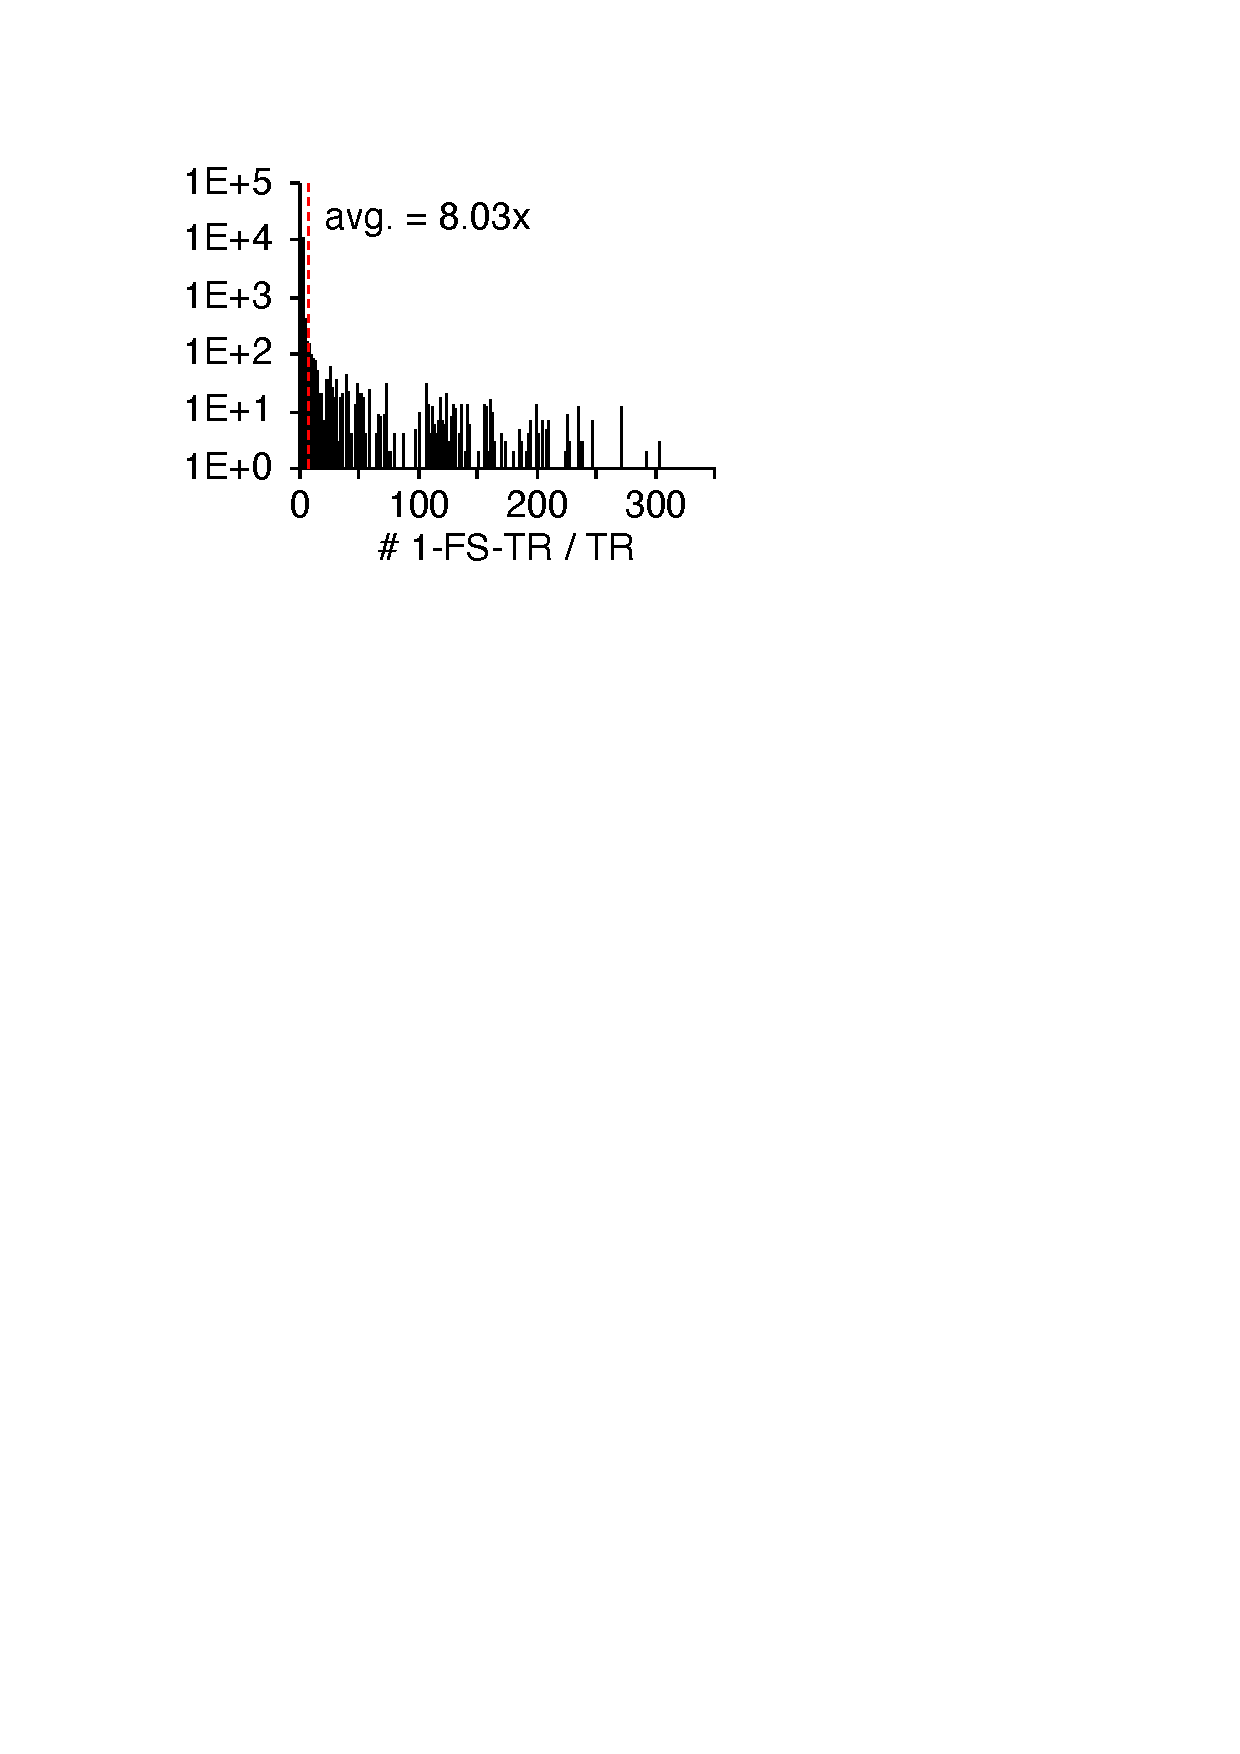
\includegraphics[width=\textwidth]{img/1-fs-hist}
    \subcaption{1-FS-TRs vs base TR.}
  \end{subfigure}
  \begin{subfigure}{0.24\textwidth}
    \centering
    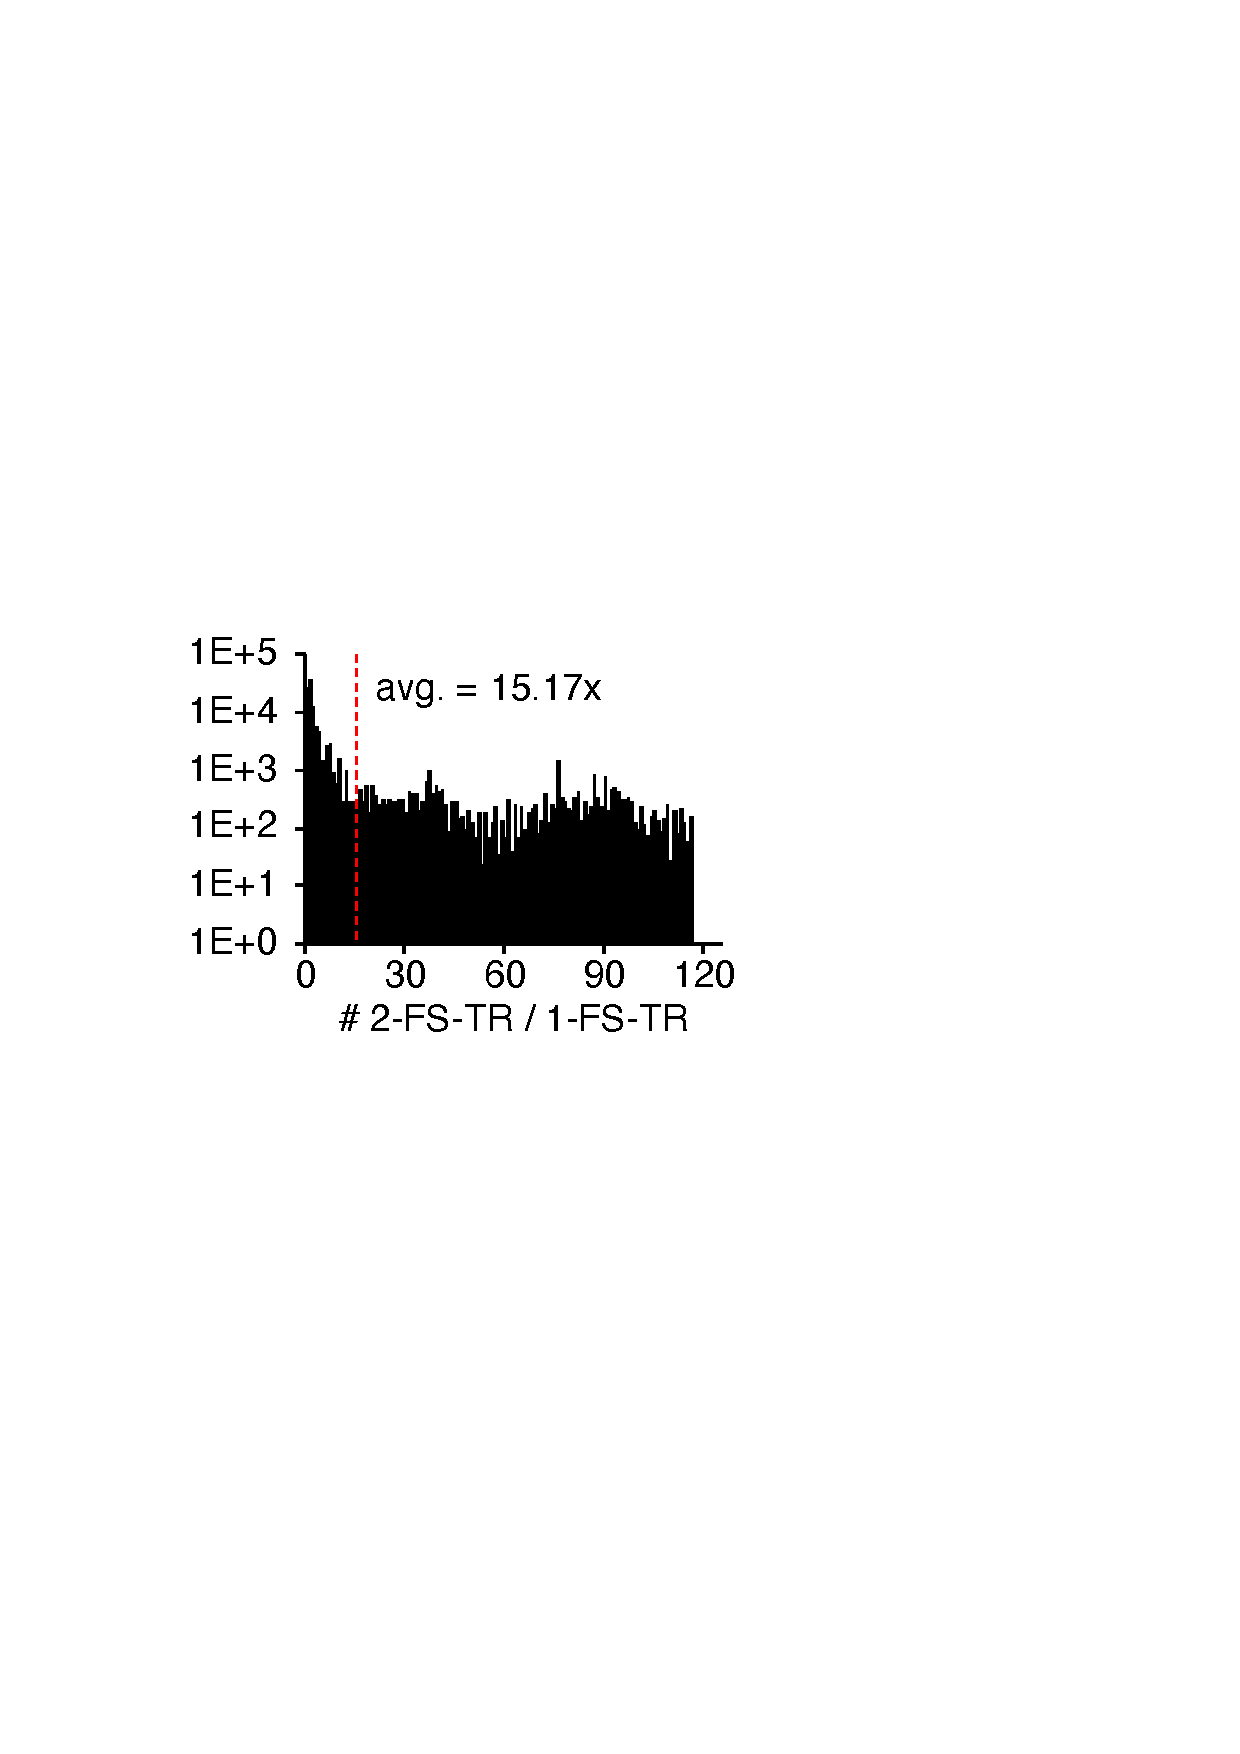
\includegraphics[width=\textwidth]{img/2-fs-hist}
    \subcaption{2-FS-TRs vs 1-FS-TR.}
  \end{subfigure}
  \begin{subfigure}{0.24\textwidth}
    \centering
    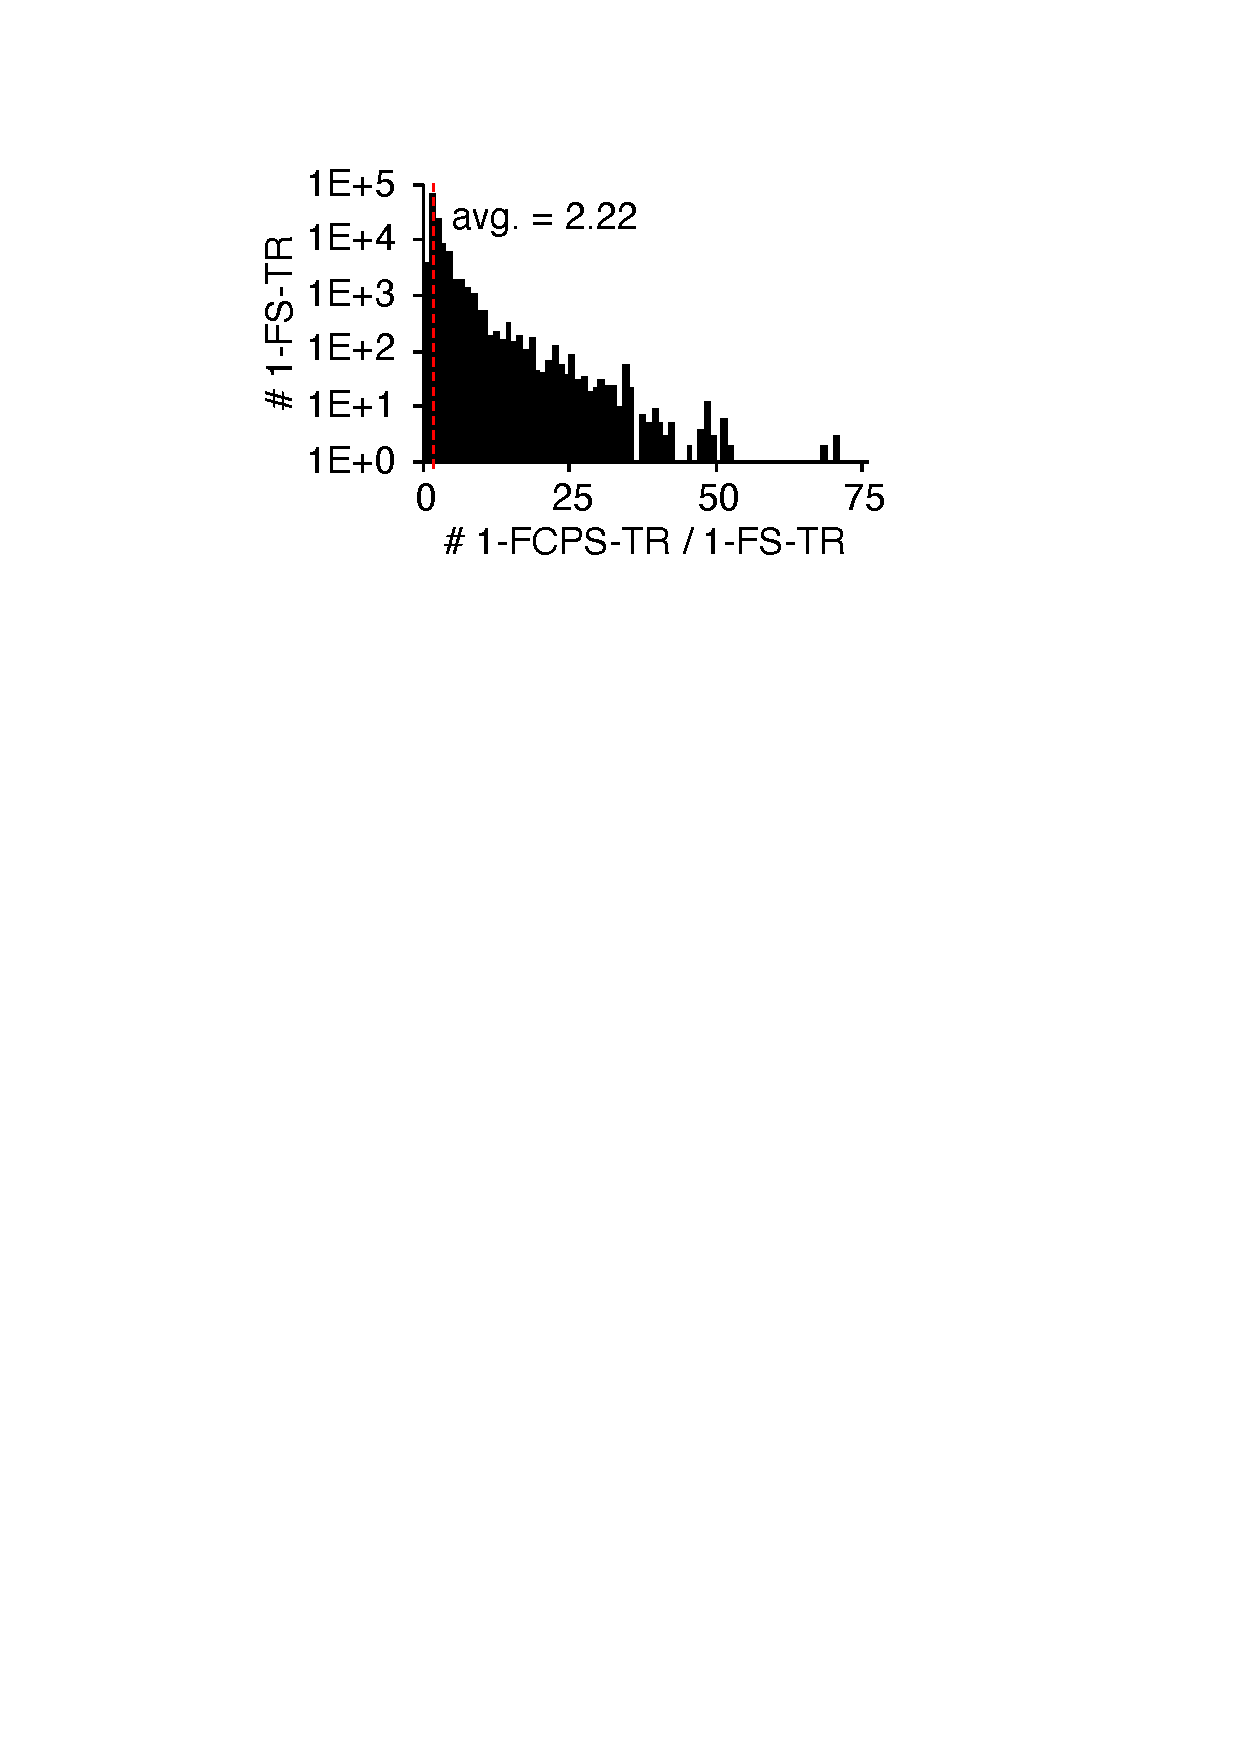
\includegraphics[width=\textwidth]{img/1-fcps-hist}
    \subcaption{1-FCPS-TRs vs 1-FS-TR.}
  \end{subfigure}
  \begin{subfigure}{0.24\textwidth}
    \centering
    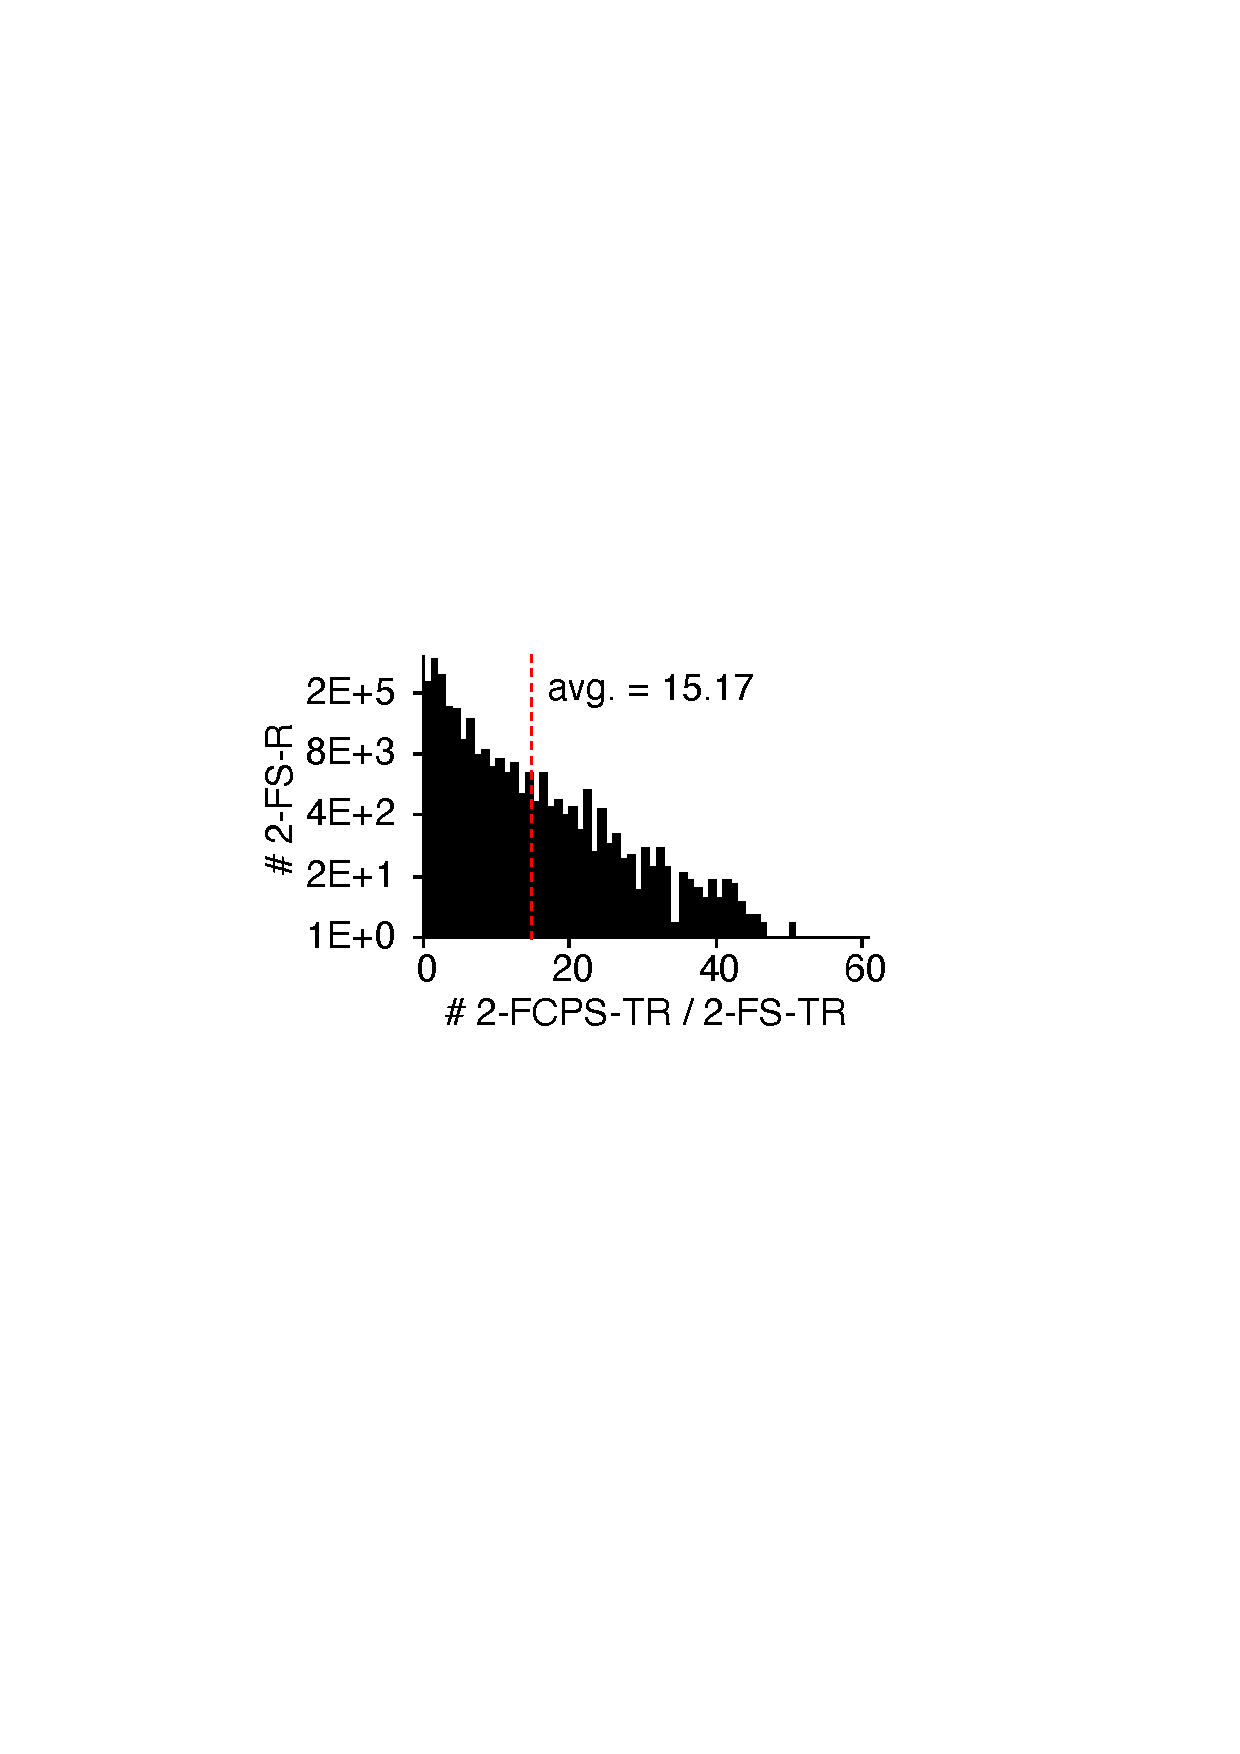
\includegraphics[width=\textwidth]{img/2-fcps-hist}
    \subcaption{2-FCPS-TRs vs 2-FS-TR.}
  \end{subfigure}
  \caption{
    The histogram of numbers of $k$-FS or $k$-FCPS TRs per less sensitive $k$-FS
    or $k$-FCPS TR.
  }
  \label{fig:hist}
\end{figure}

%----------------------------------------%

We also evaluate the impact of $k$-FCPS coverage criteria compared to $k$-FS
coverage criteria.
%
According to Table~\ref{tab:compare}, the number of covered 1-FCPS- and
2-FCPS-TRs are 277.3K and 3,620.7K, respectively.
%
Thus, 2.22 (277.3K / 125.0K) 1-FCPS-TRs exist per each 1-FS-TR, and 1.91
(3,620.3K / 1,896.1K) 2-FCPS-TRs exist per each 2-FS-TR on average.
%
It means that they are 2.22 and 1.91 feature-call-paths exist from the innermost
language features to nodes or branches in each 1-FS-TR and 2-FS-TR,
respectively.
%
For a more detailed information, we also draw a histogram of the number of
covered 1-FCPS-TRs (or 2-FCPS-TRs) per each covered 1-FS-TR (or 2-FS-TR) in
Figures~\ref{fig:hist} (c) and (j).
%
The most significant number of covered 1-FCPS-TRs per 1-FS-TR is 70 for a node
in the \jscode{Array.prototype.splice} built-in method.
%
It is a powerful built-in API feature that changes the contents of an array by
removing or replacing existing elements and/or adding new elements in place.
%
Thus, its semantics is quite complex and uses diverse helper functions, and the
number of possible feature-call-paths in this featuere is much larger than
others.
%
The most significant number of 2-FCPS-TRs per 2-FS-TR is 53 for a node whose
innermost enclosing feature is a syntactic feature for \jscode{yield} expressions
because it touches various helper functions for asynchronous behaviors.
%
Because of the increased number of TRs, the number of synthesized tests also
increased 1.34x (9,092 / 6,766) from 0-FS to 1-FS coverage criteria and 1.26x
(122,569 / 9,092) from 1-FS to 2-FS coverage criteria.
%
In addition, the number of detected unique bugs also increased when using
$k$-FCPS coverage criteria than $k$-FS coverage criteria.
%
The conformance tests synthesized with 1-FCPS and 2-FCPS coverage criteria
detected 4 (88 - 84) and \inred{4 (88 - 84)} more conformance bugs than
1-FS and 2-FS coverage criteria, respectively.
%
Now, we introduce a conformance bug example to show the impact of $k$-FCPS
coverage criteria compared to the $k$-FS coverage criteria.

%----------------------------------------%

\paragraph{\textbf{\jscode{String.prototype.normalize}}}
%
The \jscode{String.prototype.normalize} built-in API normalizes a given string
into the normalization form named by a given argument.
%
For example, \jscode{"abc".normalize("NFC")} produces the NFC normalization form
of \jscode{"abc"}.
%
If an invalid name, such as an empty string \jscode{""}, is given as the
argument, it should throw a \textbf{RangeError} exception.
%
However, the following program noramlly terminates in GraalJS v22.2.0:
\begin{lstlisting}[style=JS, basicstyle=\footnotesize\ttfamily]
String.prototype.normalize.call(0, ""); // Expected: RangeError
\end{lstlisting}
%
While this program covers a specific in \textbf{ToString} algorithm, the
semantics of this built-in API also covers that branch when converting the
\jscode{this} value.
%
It means that there are two different feature-call-path from this built-in
feature to the branch in \textbf{ToString} algorithm, and we cannot keep this
program when using $k$-FS coverage criteria even with a high $k$ value.
%
On the other hand, such feature-call-paths could discriminate two different
invocations of the \textbf{ToString} algorithm, and we successfully detected
this conformance bug with 1-FCPS and 2-FCPS coverage criteria.


%----------------------------------------%
%----------------------------------------%

\subsection{Comparison with Test262}\label{sec:compare-test262}

\begin{figure}
  \centering
  \begin{subfigure}{0.19\textwidth}
    \centering
    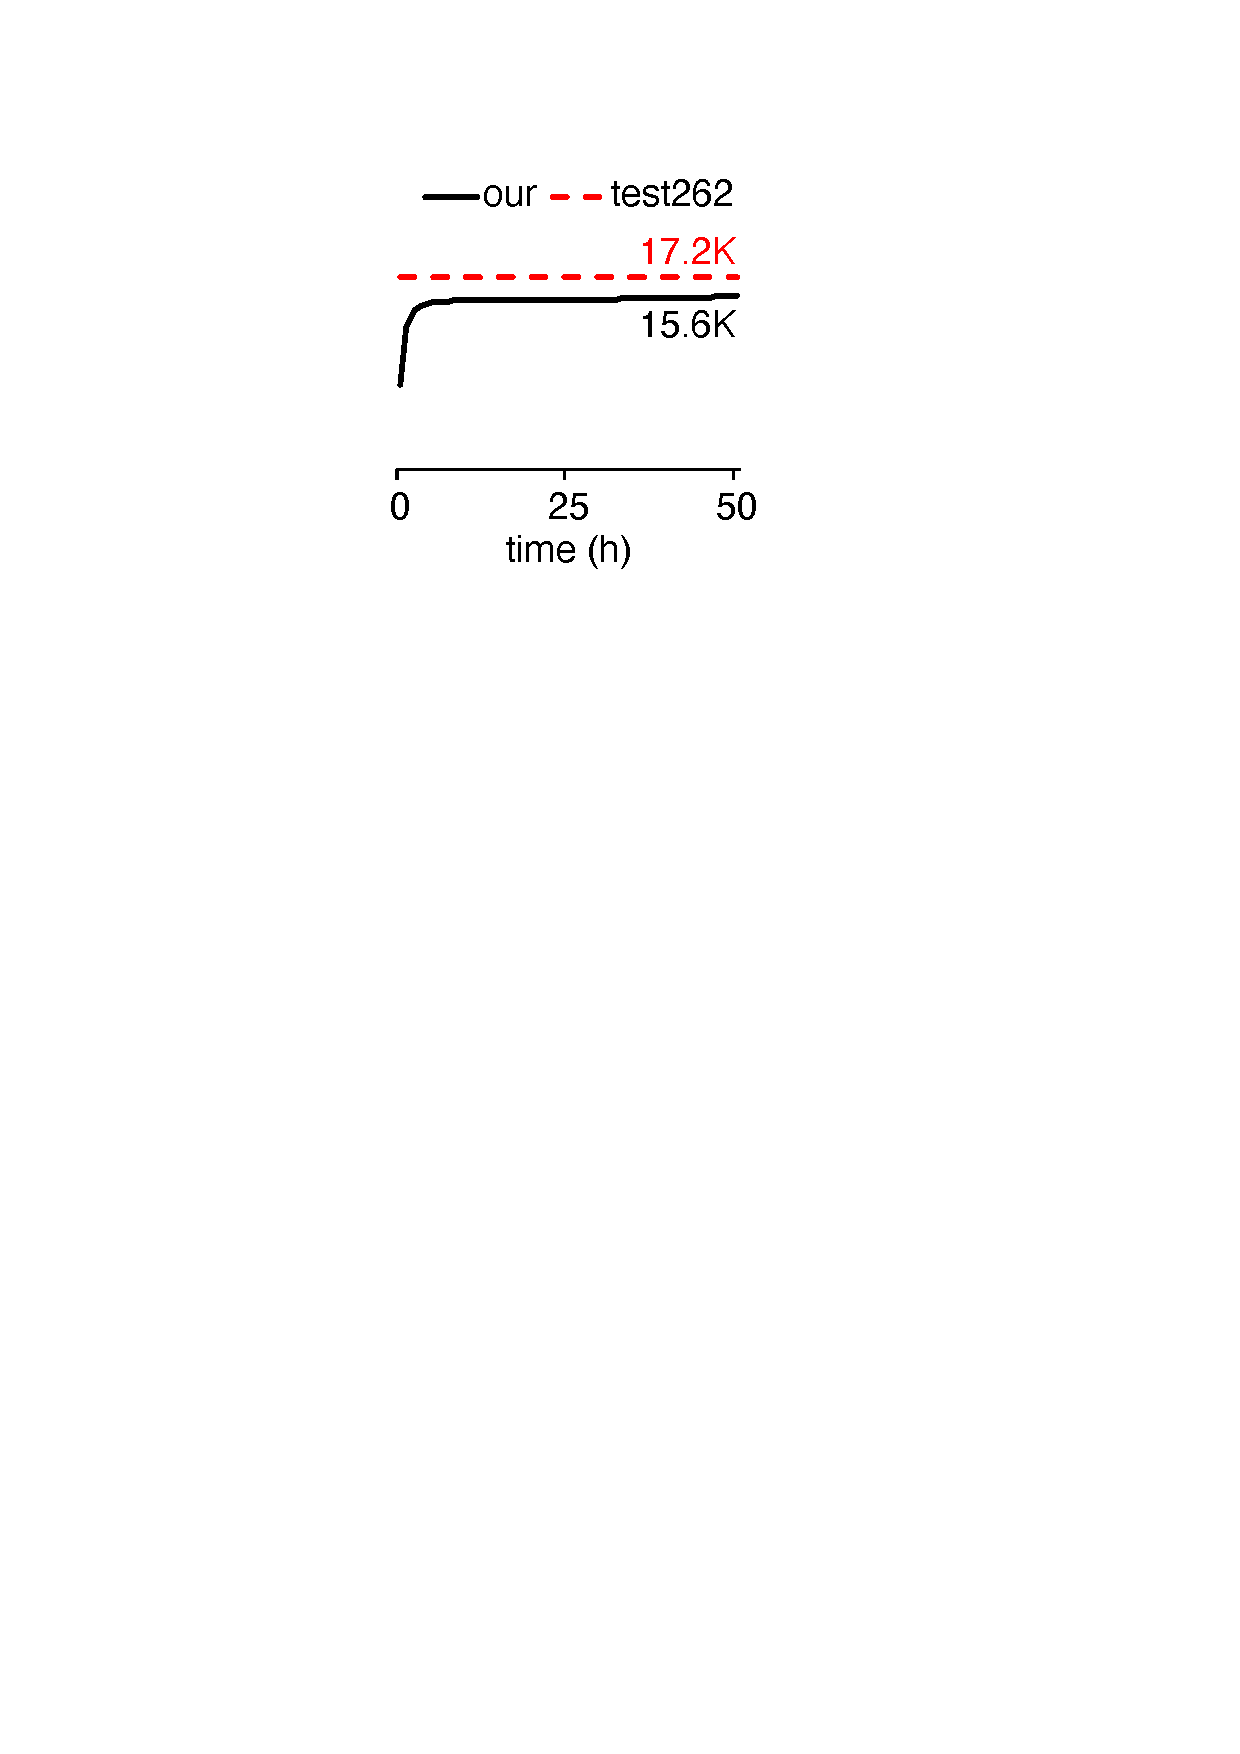
\includegraphics[width=\textwidth]{img/cov-0}
    \subcaption{Baseline.}
  \end{subfigure}
  \begin{subfigure}{0.19\textwidth}
    \centering
    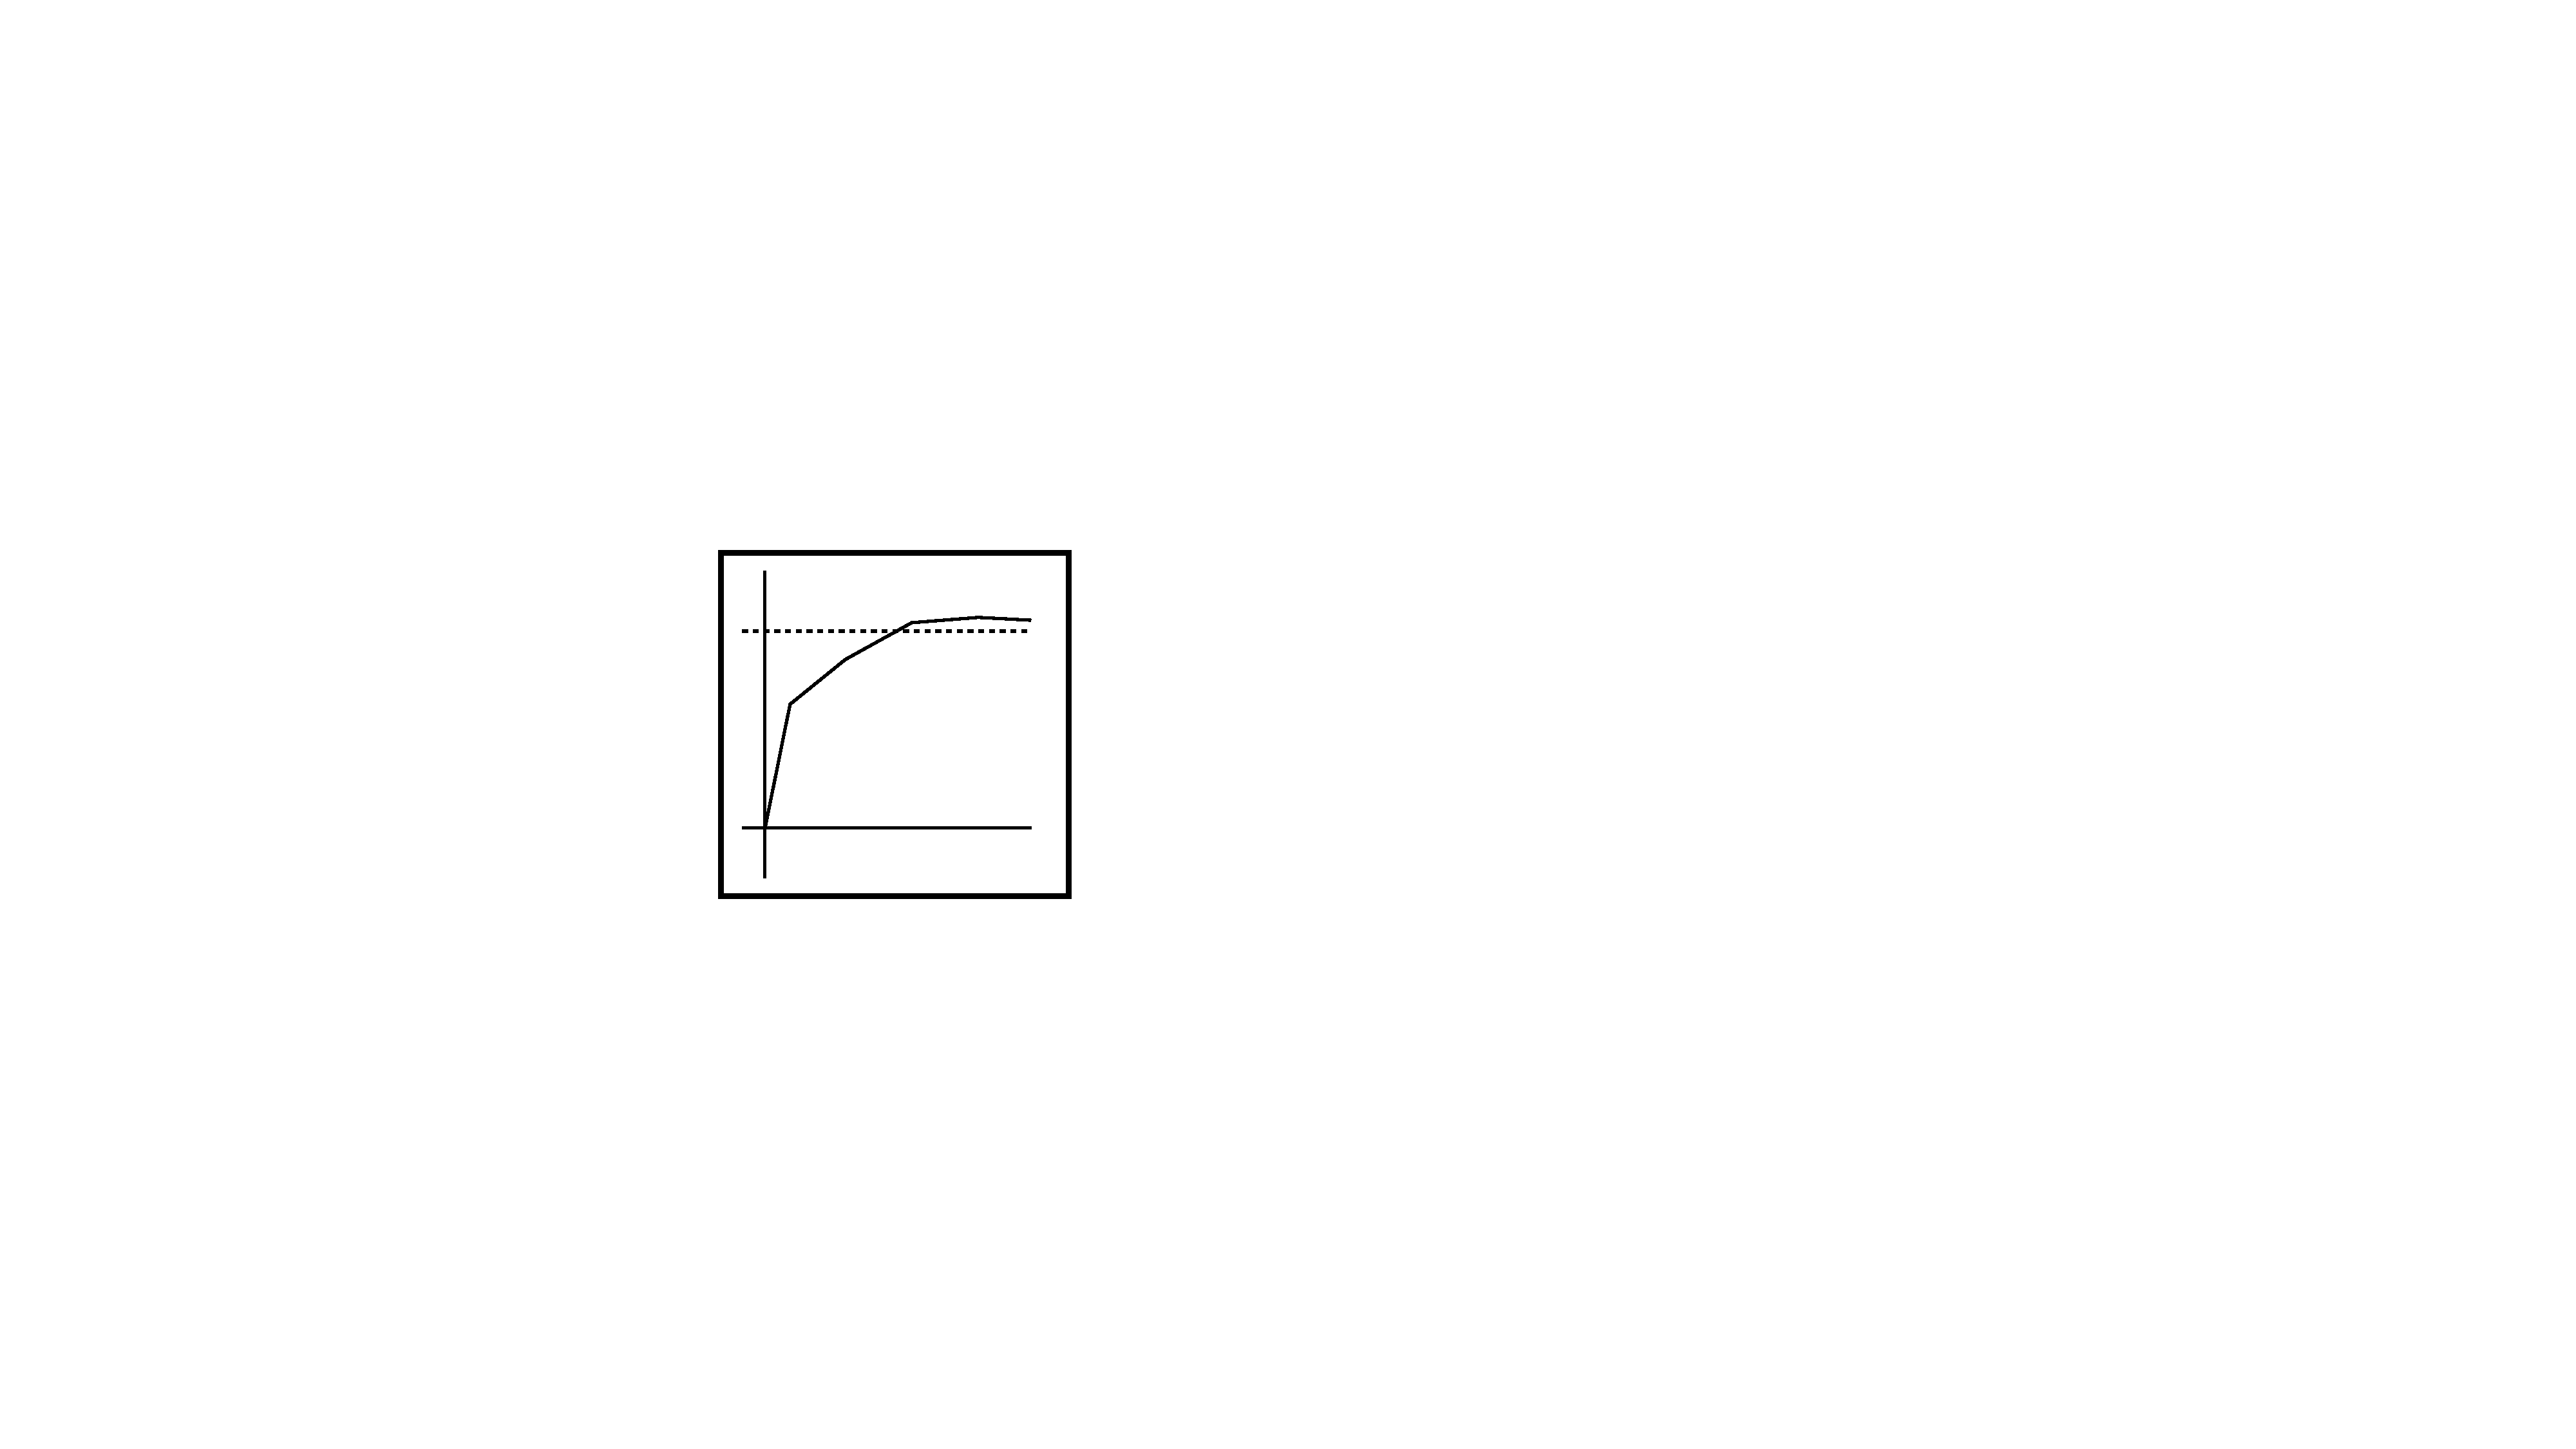
\includegraphics[width=\textwidth]{img/cov-1}
    \subcaption{1-FS}
  \end{subfigure}
  \begin{subfigure}{0.19\textwidth}
    \centering
    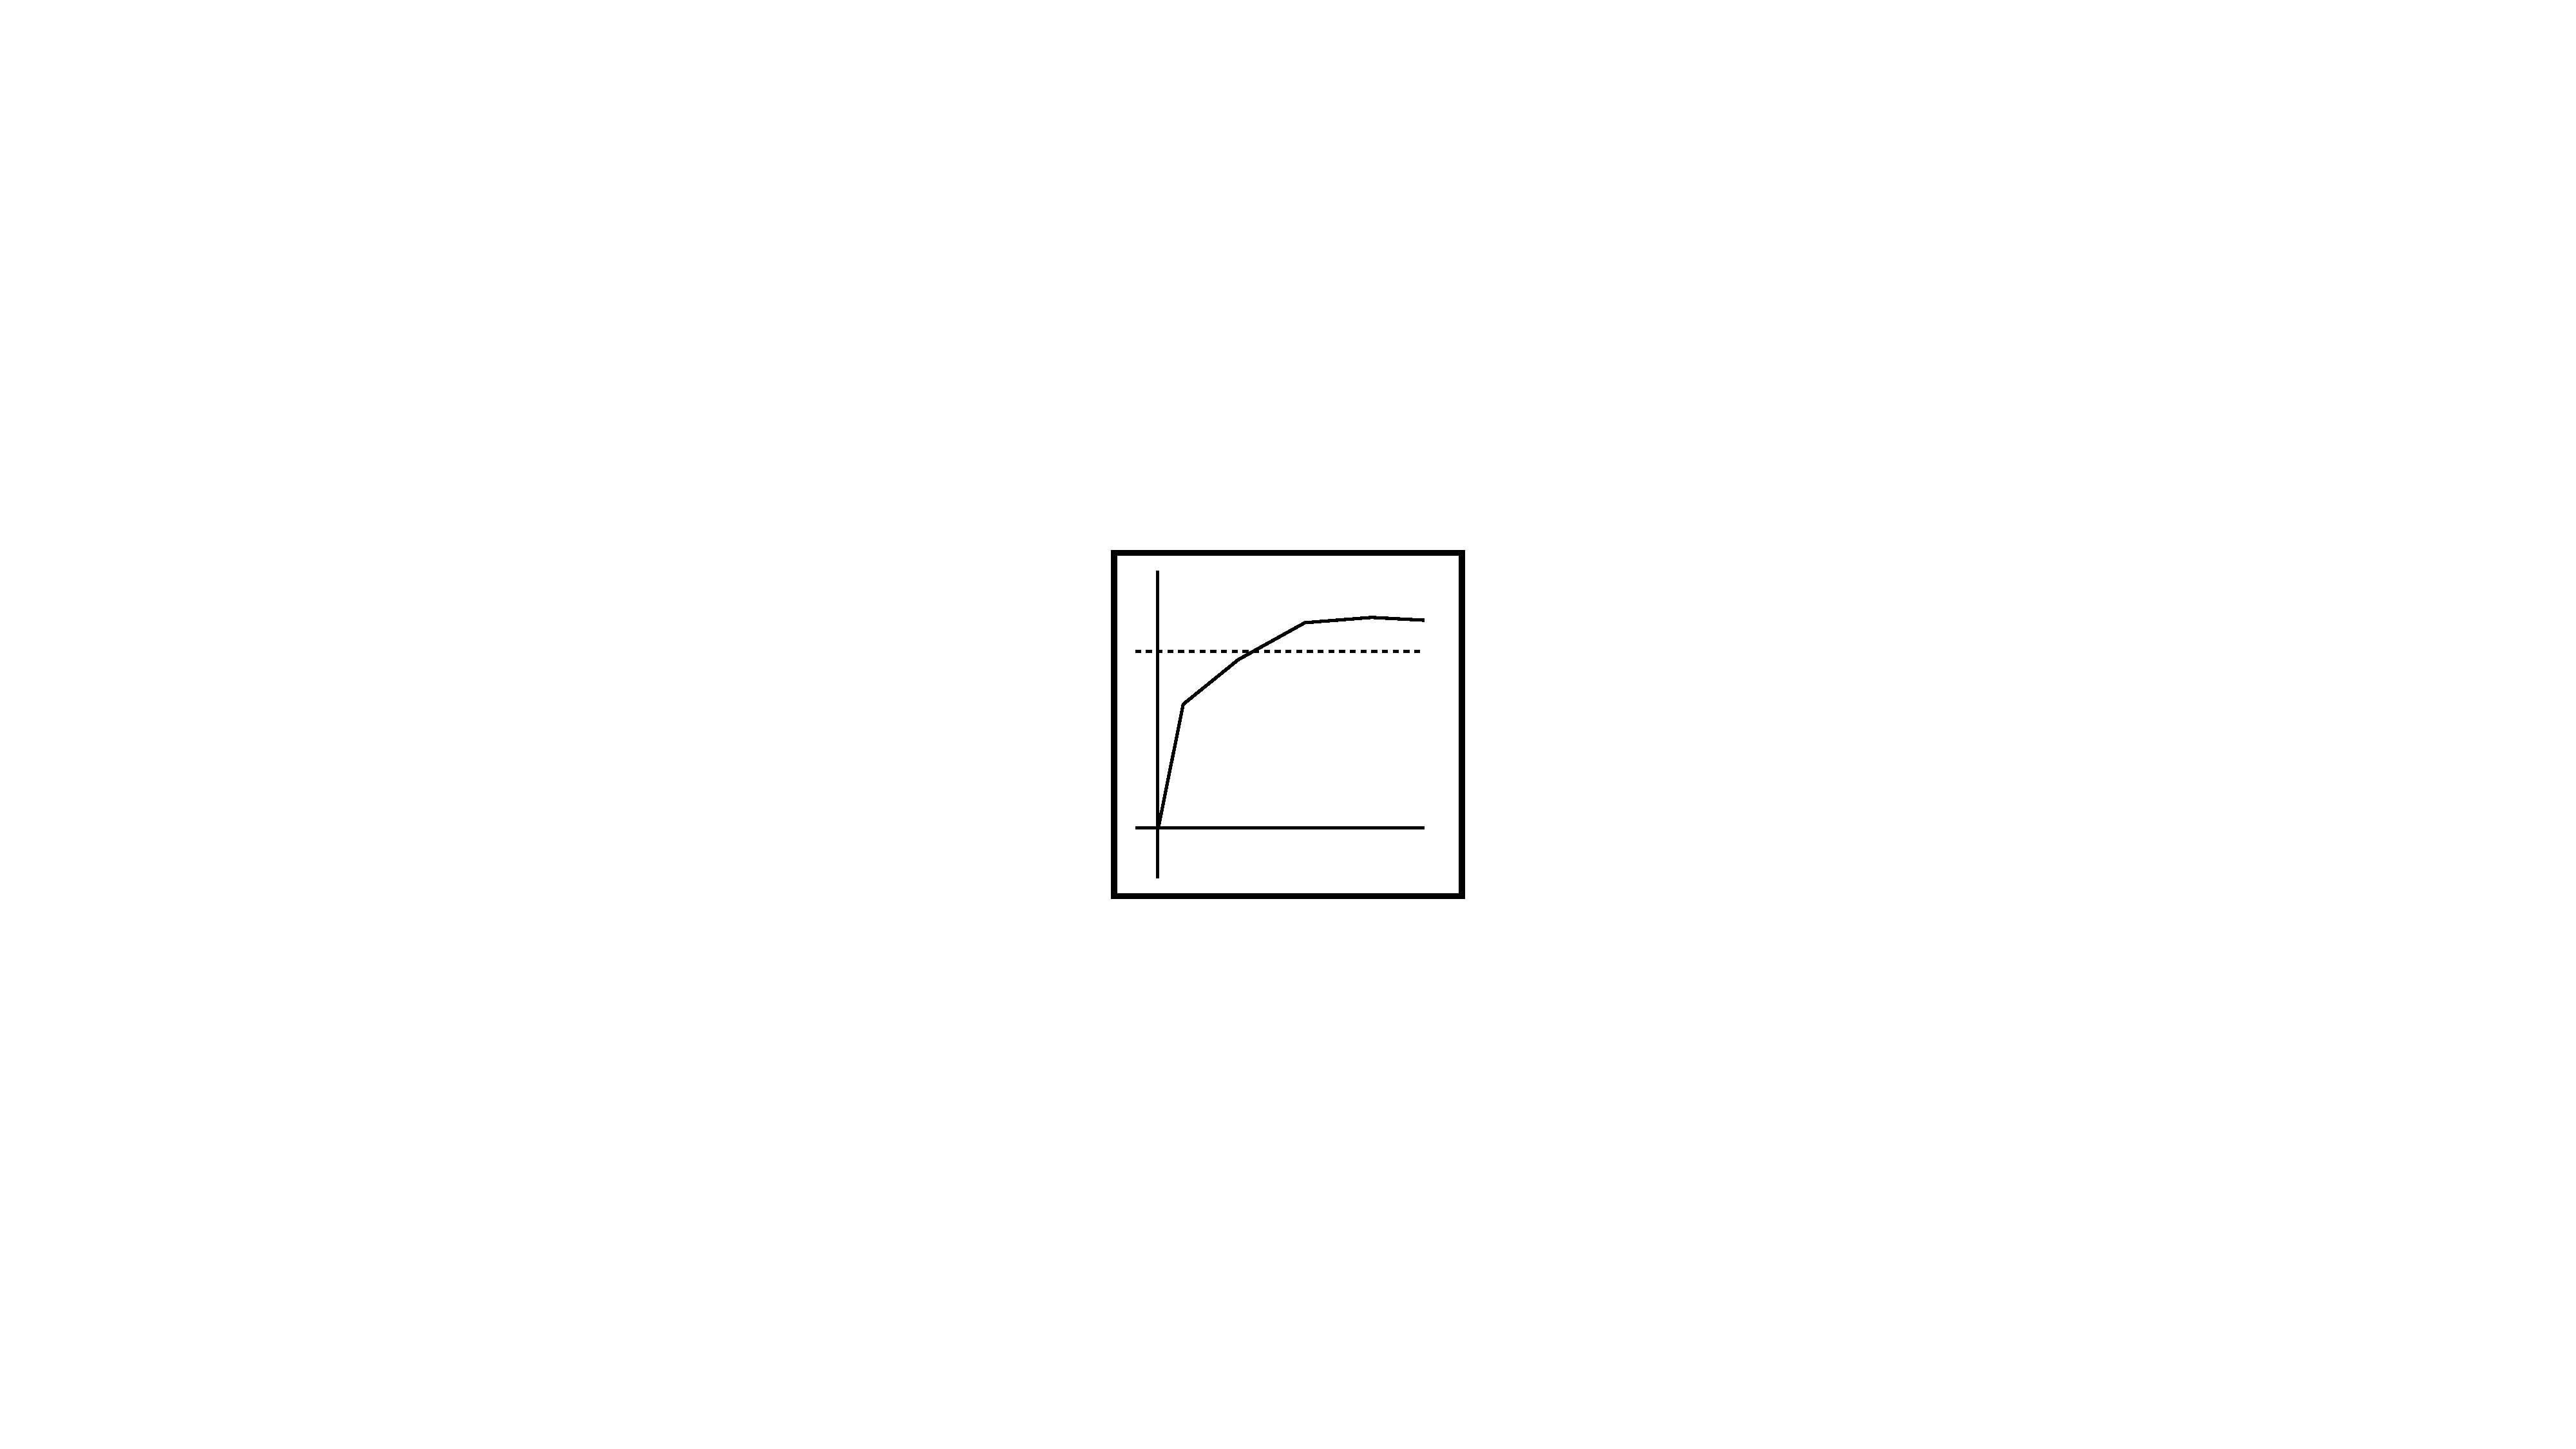
\includegraphics[width=\textwidth]{img/cov-1-fcp}
    \subcaption{1-FCPS}
  \end{subfigure}
  \begin{subfigure}{0.19\textwidth}
    \centering
    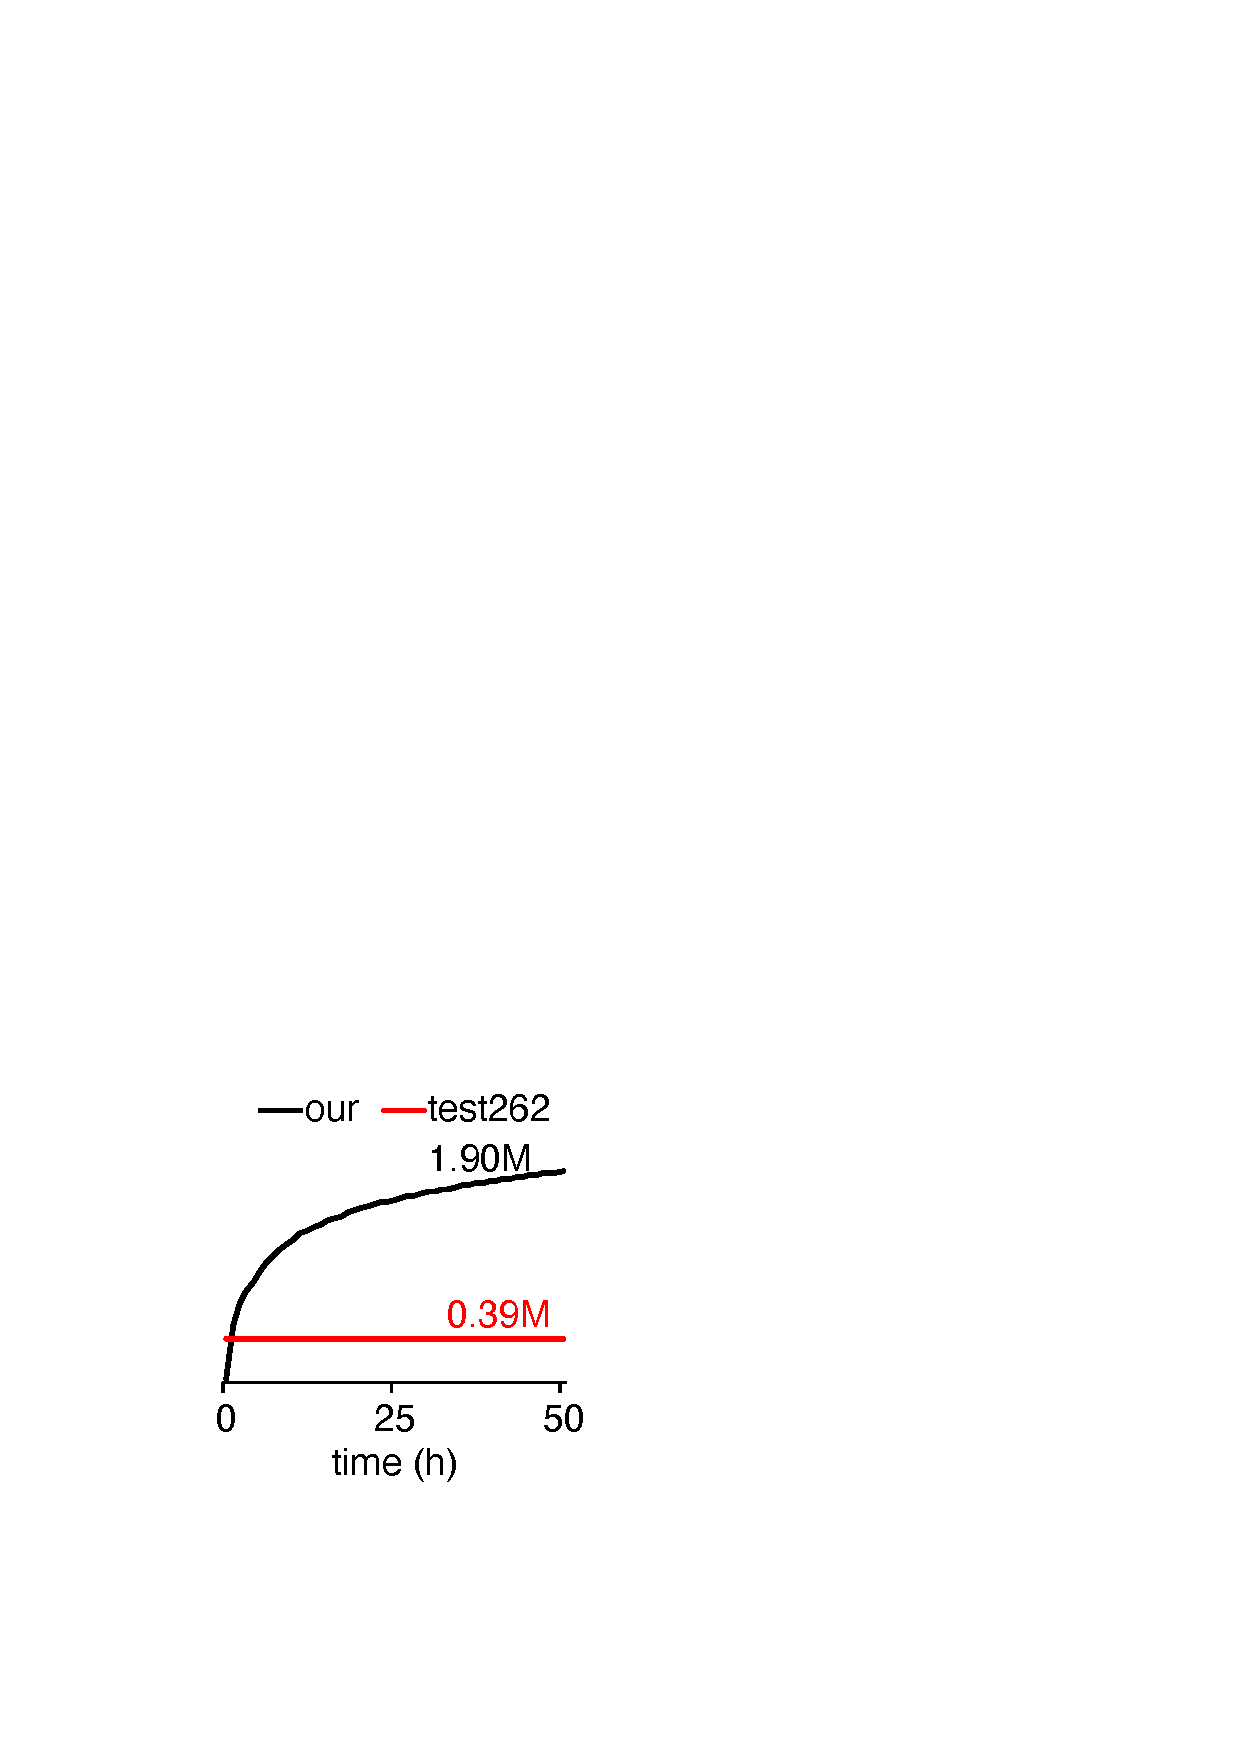
\includegraphics[width=\textwidth]{img/cov-2}
    \subcaption{2-FS}
  \end{subfigure}
  \begin{subfigure}{0.19\textwidth}
    \centering
    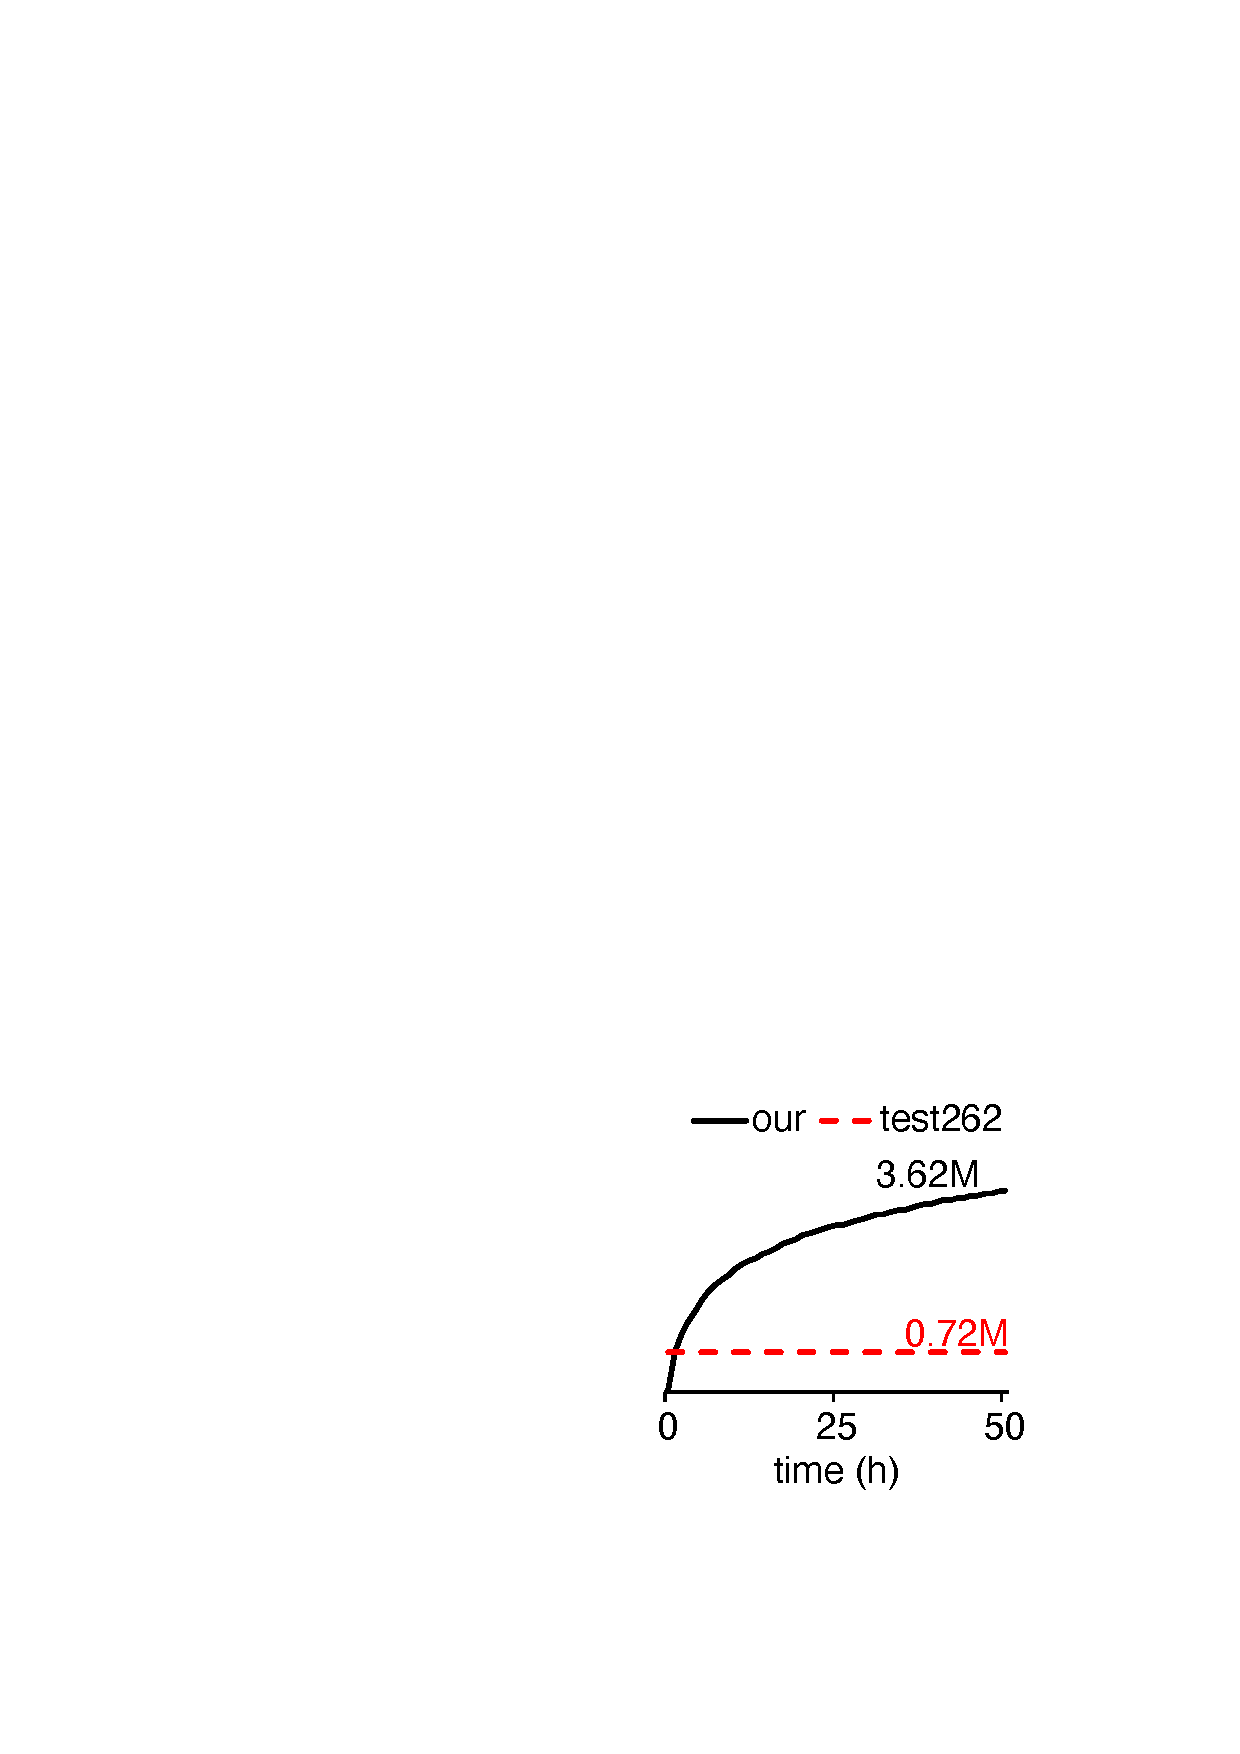
\includegraphics[width=\textwidth]{img/cov-2-fcp}
    \subcaption{2-FCPS}
  \end{subfigure}
  \caption{
    The changes of $k$-FS and $k$-FCPS node-or-branch coverage criteria with
    elapse of time.
  }
  \label{fig:cov-time}
\end{figure}

%----------------------------------------%

\begin{figure}
  \centering
  \begin{subfigure}{0.19\textwidth}
    \venn{\x{2.7K}}{\x{14.5K}}{\x{1.0K}}
    {0.15}{0.80}{0.05}
    \subcaption{Baseline.}
  \end{subfigure}
  \begin{subfigure}{0.19\textwidth}
    \venn{\x{19.3K}}{\x{69.4K}}{\x{26.3K}}
    {0.17}{0.60}{0.23}
    \subcaption{1-FS}
  \end{subfigure}
  \begin{subfigure}{0.19\textwidth}
    \venn{\x{128.8K}}{\x{213.4K}}{\x{114.7K}}
    {0.28}{0.47}{0.25}
    \subcaption{1-FCPS}
  \end{subfigure}
  \begin{subfigure}{0.19\textwidth}
    \venn{\x{146.2K}}{\x{206.2K}}{\x{1.6M}}
    {0.07}{0.10}{0.82}
    \subcaption{2-FS}
  \end{subfigure}
  \begin{subfigure}{0.19\textwidth}
    \venn{\x{612.4K}}{\x{304.4K}}{\x{3.3M}}
    {0.15}{0.07}{0.78}
    \subcaption{2-FS}
  \end{subfigure}
  \caption{
    Venn diagrams of covered TRs of $k$-FS and $k$-FCPS node-or-branch coverage
    criteria for Test262 and synthesized tests via $\tool$.
  }
  \label{fig:venn-test262}
\end{figure}


%----------------------------------------%

We compare the coverage criteria of conformance tests automatically synthesized
via $\tool$ with that of Test262, the official JavaScript conformance test
suite.
%
As described in Section~\ref{sec:impl}, $\tool$ is based on $\esmeta$ and only
targets the language features supported in the tool.
%
Thus, we removed \inred{23,231} out of \inred{47,141} conformance tests in
Test262 that utilize language features not supported in $\esmeta$ for a fair
comparison.
%
We measured five different $k$-FS and $k$-FCPS node-or-branch coverage criteria
for \inred{23,910} applicable conformance tests.
%
Figure~\ref{fig:cov-time} shows the change of $k$-FS-TPs and $k$-FCPS-TPs with
elapse of time, and the dotted line shows the coverage of Test262 in each
criterion.
%
Figure~\ref{fig:venn-test262} depicts Venn diagrams of covered TRs of $k$-FS and
$k$-FCPS node-or-branch coverage  for Test262 and synthesized tests via $\tool$.
%
In the baseline, the coverage of synthesized tests is less than that of Test262,
and covers only \inred{1.0K} TRs that not covered by Test262.
%
However, the coverage of synthesized exceeds the coverage of Test262 when using
feature-sensitive coverages.
%
In addition, the number of TRs only covered by synthesized tests also increases,
and the conformance tests synthesized with $2$-FCPS-TRs cover \inred{3.3M}
2-FCPS-TRs not covered by Test262.
%
We believe that this is why $\tool$ successfully detected diverse new bugs in
existing JavaScript engines and transpilers, even though most of them are
heavily tested using Test262.
